% !TEX root = ../my-thesis.tex
%
\chapter{ESTADO DEL ARTE}
\label{sec:estado del arte}

En este capítulo se tratará de realizar una revisión del estado del arte. Se tocará el estado actual en el que se encuentra la agricultura, la tendencia hacia técnicas de agricultura de precisión. De aquí, se desarrollará la importancia de discriminar entre diferentes tipos de vegetación para su tratamiento individualizado y se verán cuales han sido las tecnologías y técnicas empleadas históricamente para este proceso.

\section{Agricultura}

La agricultura es la actividad ocupada en el cultivo del suelo y la recogida posterior de las cosechas; es una de las grandes invenciones del hombre, que permitió a la civilización un acceso sencillo a los alimentos, permitiendo pasar a sociedades sedentarias como las que conocemos en la actualidad. Esta es una de las principales actividades del sector primario.

Durante el desarrollo de la agricultura, se han visto numerosas revoluciones y transformaciones a lo largo de los años, debido al avance de la tecnología y a las necesidades de la población existente en cada zona del planeta. De entre las más recientes, se puede destacar la vivida en la segunda mitad del siglo XX, donde, por un gran crecimiento de la población trajo un aumento en la demanda de alimentos. Es por ello que se tuvieron que implementar nuevas tecnologías en el campo \cite{Shuler2003}, como pudo ser el uso del tractor, tal y como se conoce en la actualidad, lo que supuso una reducción notable de la mano de obra necesaria para el trabajo en el campo. Además, debido a la mejora en químicos como herbicidas y pesticidas o fertilizantes artificiales, la productividad de los cultivos aumentó considerablemente, adaptándose la producción a las necesidades de la época.

Como contrapartida a esto, este tipo de técnicas han supuesto un deterioro muy importante en la calidad del medioambiente con el vertido de este tipo de productos de forma incontrolada.

En la actualidad, tal y como apuntan varios informes \cite{fao_agricultura_2020} \cite{food2004agricultura} en los últimos años por la FAO (\textit{Food and Agriculture Organization of the United Nations}), en los próximos años se podrá observar una gran transformación en la agricultura y en la alimentación de las personas. Esto se debe, en primer lugar, a la necesidad de una agricultura más sostenible con el medio ambiente. En segundo lugar, debido a las notables consecuencias del cambio climático en el planeta, la variabilidad del clima y de las precipitaciones que supondrán un problema que habrá que enfrentar, para lo que será necesaria la transformación de algunas de las técnicas empleadas actualmente. 

Además de todo lo anterior, otro punto a tener en cuenta es el continuo crecimiento poblacional mundial, crecimiento que podrá suponer un problema para el acceso a los alimentos en los próximos años si no es posible encontrar mejores alternativas con las que trabajar el campo.

\section{Agricultura de Precisión}

La agricultura de precisión se basa en la gestión heterogénea de los cultivos con el fin de aumentar la productividad. En este ámbito, se debe analizar la variabilidad de estos durante las diferentes etapas de su desarrollo. Alguno de los ejemplos que se pueden encontrar en este ámbito son: el estimar la densidad de sembrado, analizar y calcular la cantidad adecuada de fertilizantes, aplicar de forma óptima herbicidas para malas hierbas o analizar el estado actual y el rendimiento de los cultivos.

La \textit{International Society of Precision Agriculture} propone otra definición, mucho más exacta: \textit{``La agricultura de precisión es una estrategia de gestión que recoge, procesa y analiza datos temporales, espaciales e individuales y los combina con otras informaciones para respaldar las decisiones de manejo de acuerdo con la variabilidad estimada, y así mejorar la eficiencia en el uso de recursos, la productividad, la calidad, la rentabilidad y la sostenibilidad de la producción agrícola.''} \cite{ispa}

Sus orígenes se remontan a principios de los años 80 en los Estados Unidos \cite{Robert2002}, donde se comienza con el uso de las nuevas tecnologías disponibles para mejorar la aplicación de fertilizantes en cantidades variables según las necesidades de los cultivos. Posteriormente, esto fue extendiéndose a diferentes prácticas y países. 

La principal motivación del uso de agricultura de precisión proviene de la variabilidad de los cultivos, que puede venir dada desde diferentes puntos. Por ejemplo, la variabilidad producida por el entorno en el que está situado el cultivo, la variabilidad producida por las condiciones climáticas o la producida de manera intencional al utilizar fertilizantes.

Actualmente este tipo de técnicas son una realidad, sin embargo siguen existiendo numerosas barreras tecnológicas que se están tratando de erradicar para poder llevar a cabo este tipo de prácticas de forma satisfactoria. Esto se debe a que el número de tecnologías que se involucran dentro de este tipo de agricultura es muy alto, ya que se necesita obtener gran información del campo. En esta se emplean tecnologías como el uso de sistemas de posicionamiento global (GPS), sensores capaces de monitorizar el estado de las plantas o maquinaría capaz de actuar en las zonas objetivo. \cite{Garcia2008}

\begin{figure}
    \centering
    \includegraphics[width=\textwidth]{figuras/estado del arte/dron_inspeccion.jpg}
    \caption{UAV de inspección en Agricultura de Precisión para floricultura en Alemania}
    \label{fig:dron_inspeccion}
\end{figure}

En la Figura \ref{fig:dron_inspeccion}, se puede ver un ejemplo de aplicación de UAVs para la inspección de cultivos de flores en Alemania \cite{job-wizards}. Aquí se combinan tecnologías basadas en el desarrollo de vehículos aéreos no tripulados, la sensorificación a partir de cámaras RGB para la obtención del estado de las plantas, el posicionamiento GPS del vehículo y las comunicaciones en tiempo real de este.

La agricultura de precisión trae asociada numerosos beneficios frente a otros tipos de agricultura. Esta tiene como objetivo principal aportar mas información a los agricultores sobre el estado y la variabilidad de su parcela de cultivo, lo que servirá para conocer cuales son las necesidades reales del campo para su posterior labrado, siembra, riego, fertilización, control de plagas o tratamiento de malas hierbas. Esto trae consigo una mejora en la explotación de la parcela, una reducción en costes y un menor impacto medioambiental.

Enumerando alguno de los beneficios, podemos encontrar los siguientes \cite{Garcia2008}:
\begin{itemize}
    \item Gestión optimizada de las explotaciones.
    \item Reducción de la aplicación de fertilizantes, herbicidas y pesticidas.
    \item Productos con mayor valor nutritivo.
    \item Menor impacto para el medio ambiente.
    \item Reducción en el uso de combustibles para la maquinaria agrícola.
    \item Obtención de información de los cultivos más precisa y con mayor trazabilidad.
\end{itemize}

\section{Tratamiento selectivo contra malas hierbas}

Dentro de la agricultura de precisión, una de las técnicas que adquieren especial importancia, es la aplicación selectiva de agroquímicos \cite{precisionweedmanagement}. Al contrario que los métodos tradicionales, estos métodos proponen ajustar las dosis de tratamiento a las necesidades de cada cultivo, usándose tan solo en las áreas realmente afectadas.

Este área despierta gran interés debido a que es uno de los grandes problemas agrícolas actuales. Esto es así, ya que se estima que puede ser uno de los grandes limitadores dentro de rendimiento potencial de los cultivos. Algunos autores indican que puede llegar a ser incluso hasta un 40\% del potencial total del cultivo \cite{Oerke1999} contando la afectación de otros agentes externos. Las malas hierbas, compiten con las plantas del cultivo por los recursos de la tierra, lo que supone una gran reducción en el rendimiento del terreno.

Algunos experimentos realizados, muestran que el ahorro en agroquímicos puede suponer hasta un 80\% con el uso de estas técnicas selectivas \cite{RUIZ2006} \cite{Hamouz2018ImpactOS} con respecto a las dosis recomendadas, sin necesidad de disminuir en su eficacia ni en el rendimiento de la cosecha. Esto viene traducido en un gran ahorro en los costes de producción.

Además, esto no tiene solo un gran impacto económico, sino que tiene un gran impacto medioambiental, ya que el tratamiento de herbicidas de manera extensiva, causa la contaminación de aguas o la afectación a cultivos cercanos.

Para la aplicación selectiva de tratamiento es necesario una estimación inicial de la cantidad de producto para cada unidad de cultivo \cite{Senay1998}. Para ello, es necesario primeramente, determinar la localización, ver la densidad y clasificar los diferentes tipos de malas hierbas. Con esta información, posteriormente se realiza un selección del modo de actuación adecuada. Finalmente, se aplica de forma selectiva y precisa el tratamiento según las indicaciones estipuladas anteriormente.

\subsection{Técnicas de tratamiento}

Existen diferentes técnicas para el tratamiento de malas hierbas que compiten con el cultivo. Normalmente estas se dividen en cuatro categorías diferenciadas.

\begin{itemize}

    \item \textbf{Técnicas mecánicas:} aquellas que que se aplican directamente sobre las malas hierbas para eliminarlas. Algunas de estas son el entierro, el corte o la quema de esta vegetación.
    
    \item \textbf{Técnicas culturales:} aquellas que no emplean uso de químicos y que se realizan a partir del conocimiento de la propia tierra y el cultivo. Algunas de estas son el labrado, el uso de falsas siembras o el atraso de la fecha de siembra.
    
    \item \textbf{Técnicas biológicas:} aquellas que emplean enemigos naturales para eliminar las malas hierbas. Algunas de estas pueden ser el pastoreo, el uso de micoherbicidas o la aleopatía.
    
    \item \textbf{Técnicas químicas:} aquellas que incluyen principalmente el uso de herbicidas para la eliminación y control de malas hierbas.
    
\end{itemize}

Aún así, desde la aparición durante el siglo XX de herbicidas como ya se comentaba, las técnicas mecánicas han sido relegados a un segundo plano. Esto es debido a su eficacia y su facilidad de uso.

Gran parte de estas técnicas presentadas son empleadas de igual manera en la agricultura de precisión \cite{Weis2008}, pero para su automatización requieren de procesos automatizados de localización y aplicación precisa del tratamiento \cite{Westwood2018}, lo que no resulta trivial en la mayoría de casos debido a la realización de estas técnicas sobre terrenos poco estructurados y con gran variabilidad. Aún así, se espera que para los próximos años, estos problemas tecnológicos sean ampliamente superados y suponga una gran revolución dentro de la agricultura.

Actualmente, ya se desarrollan vehículos donde se montan diferentes herramientas de aplicación de herbicidas o de técnicas mecánicas, que de manera efectiva y selectiva, son capaces de ir eliminando estas malas hierbas sin afectar de manera notable al cultivo. Un ejemplo de esto es el autómata \textit{BoniRob}, el cuál es capaz de realizar mapeo de los campos para posteriormente eliminar las malezas que se localizan de diferentes formas en esta, tanto aplicando herbicidas \cite{Scholz2014} como técnicas de corte \cite{EvanAckerman2021}. En la Figura \ref{fig:bonirob}, se puede ver una fotografía de este autómata.

\begin{figure}[h]
    \centering
    \includegraphics[width=\textwidth]{figuras/estado del arte/bonirob.jpg}
    \caption{Fotografía del robot \textit{BoniRob} \cite{Pittman2021}}
    \label{fig:bonirob}
\end{figure}

\subsection{Técnicas de localización}

La localización y clasificación de malas hierbas dentro del cultivo es uno de los grandes retos a los que se está enfrentando desde que se desea implementar este tipo de procesos \cite{Weis2008} dentro de la agricultura de precisión.

Este técnica se puede realizar de múltiples maneras, donde las más sencilla, es la propia inspección visual de forma manual, donde una persona experta va registrando la aparición de estas. Esta técnica resulta eficiente a la hora de localizar estas plantas, pero no es soportable para grandes cultivos, debido al enorme incremento de costes por el gran volumen de mano de obra necesaria. Debido a esto por lo que actualmente se tratan de desarrollar técnicas automatizadas para la realización de este tipo de tareas.

Algunas de las técnicas más desarrolladas a día de hoy se basan en el uso de cámaras hiper-espectrales \cite{Li2021} que funcionan recopilando información en todo el espectro electromagnético, pudiendo observar espectros de la luz no visible, consiguiendo recopilar gran cantidad de información de gran valor para poder diferenciar fácilmente entre diferentes tipos de vegetaciones. En la Figura \ref{fig:hyperespectral}, se puede observar un ejemplo de imagen tomada con este tipo de cámaras.

\begin{figure}[h]
    \centering
    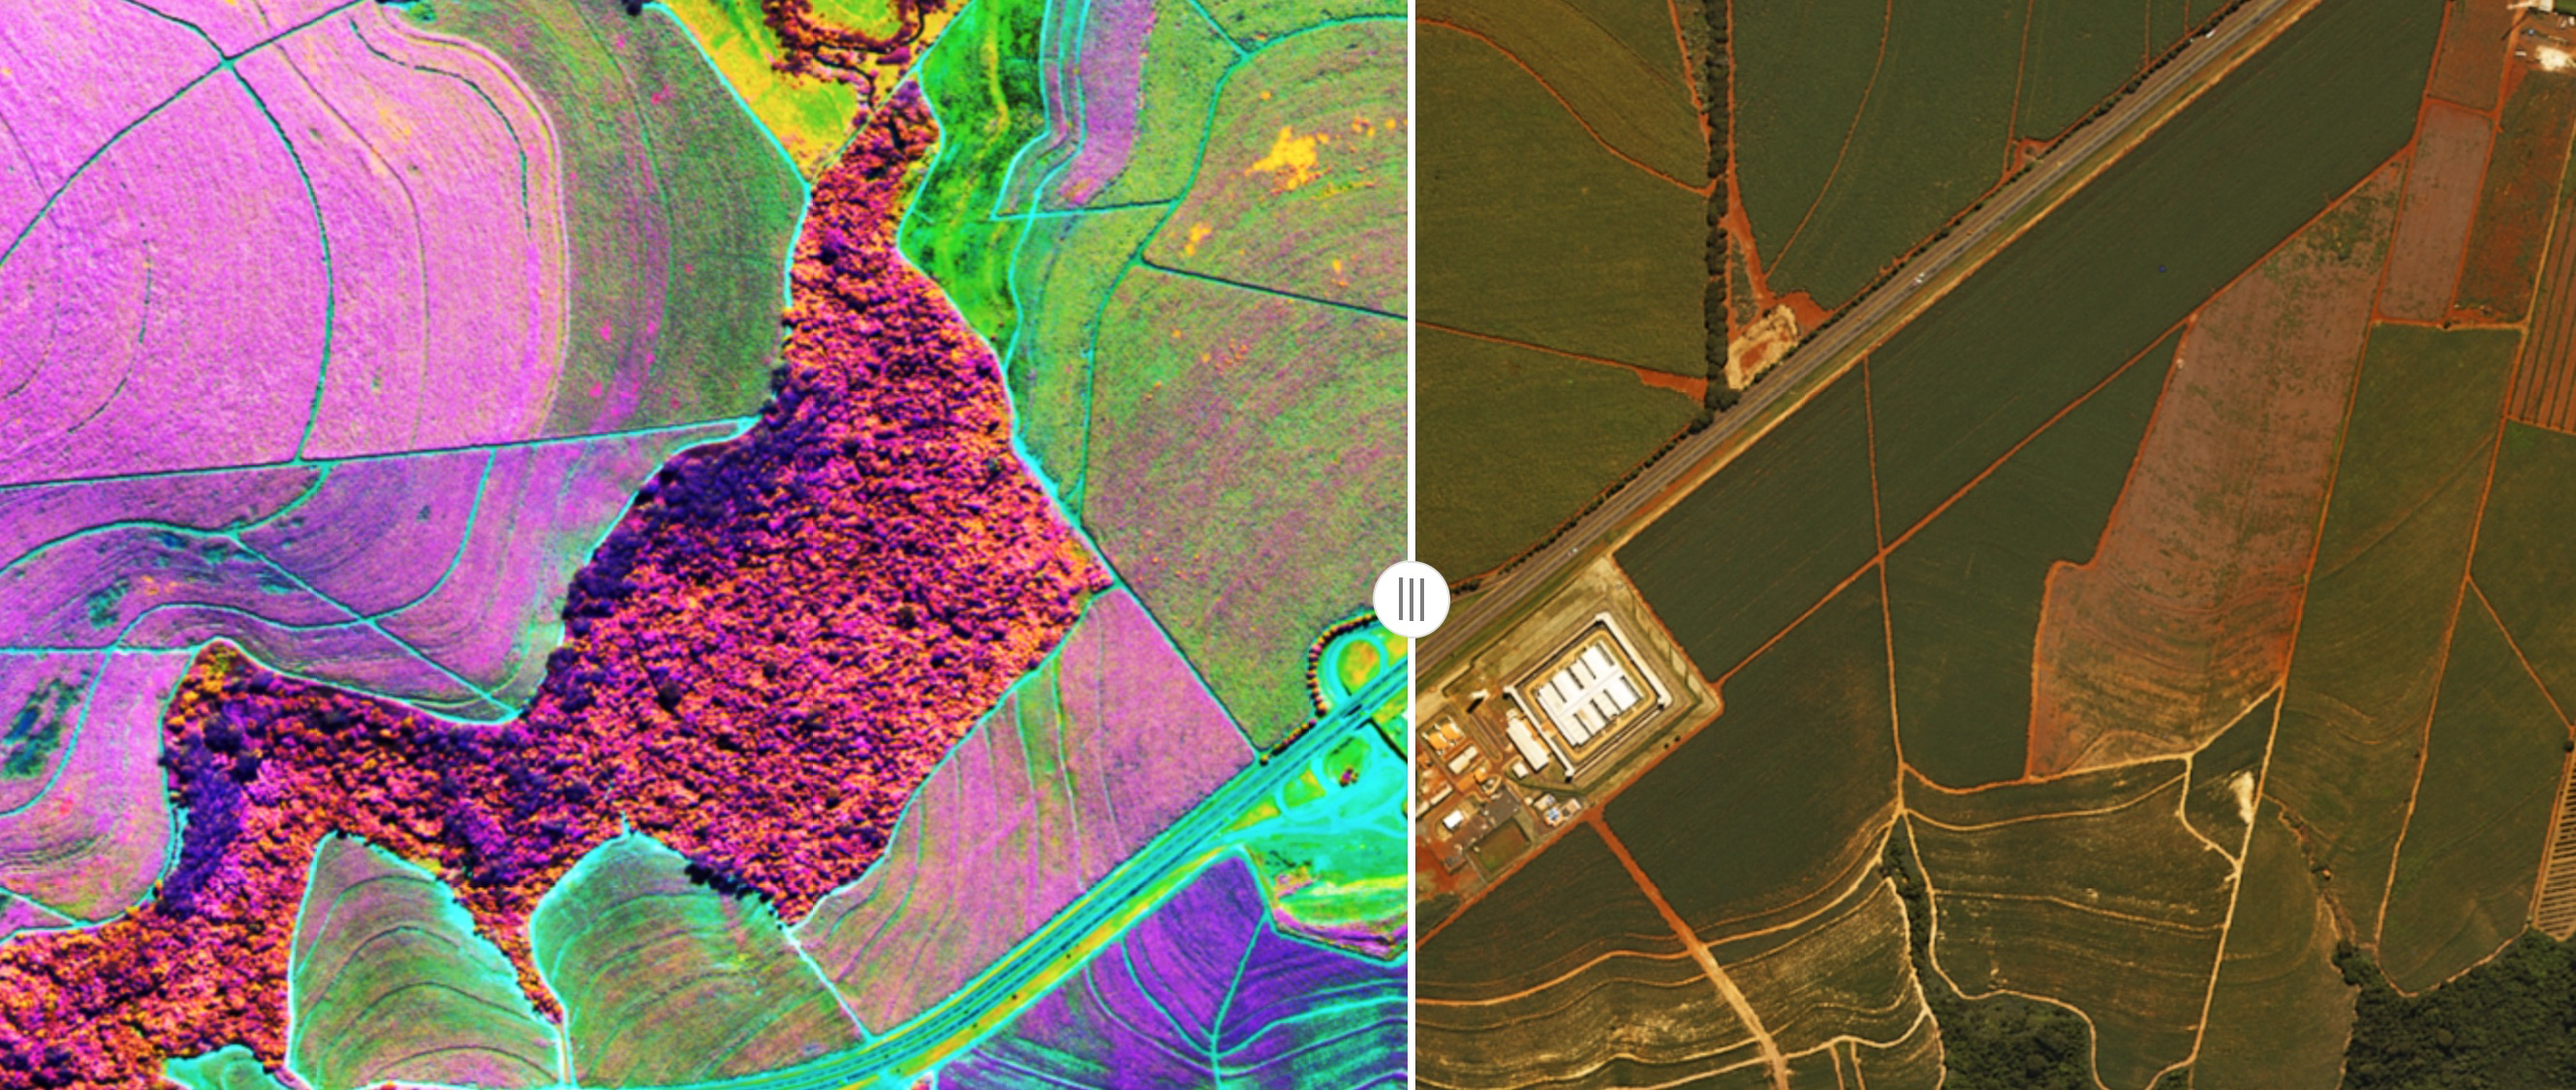
\includegraphics[width=\textwidth]{figuras/estado del arte/hyperspectral_image.png}
    \caption{Comparación de fotografía tomada con cámara hiper-espectral y con cámara RGB \cite{igor_hyperspectral_2018}}
    \label{fig:hyperespectral}
\end{figure}

A pesar de esto, en los últimos años se ha visto fuertemente desarrollado el uso de cámaras RGB, que tan sólo son capaces de ver el espectro visible de la luz, las cuales usadas junto a técnicas de segmentación y clasificación de imágenes, son capaces de diferenciar de igual manera y con gran precisión los diferentes tipos de vegetación existentes. Estas tienen la problemática de que se ven muy influenciadas por la iluminación de la escena \cite{Lameski2017}, pero por otro lado, su precio es bastante inferior a las cámaras hiper-espectrales presentadas anteriormente \cite{Gasparovic2020}, por lo que resulta altamente interesante su uso en este tipo de aplicaciones.

\section{Clasificación de Imágenes}

En los últimos años, el desarrollo de la visión por computador ha sido un hito importante en el avance del despliegue de aplicaciones de robótica y automática, de manera que sea posible comprender el entorno que nos rodea extrayendo datos relevantes de las imágenes de forma automatizada.

Uno de los bloques más relevantes dentro de este, es el desarrollo de algoritmos de clasificación de imágenes, el cual se encarga de etiquetar imágenes en función del contenido que existe en ella, extrayendo propiedades que los hagan distinguibles de otras.

Desde un punto de vista clásico, esto se ha ido realizando siguiendo una serie de pasos determinados que son: el tratamiento de la imagen, la extracción de características y la clasificación. Todos estos pasos dependían del diseñador del algoritmo y del problema que se trataba de solucionar. Es por ello que muchos de estos algoritmos se centraban en la clasificación de cierto tipo imágenes en problemas cerrados y en el que tan solo ciertas condiciones eran contempladas.

Sin embargo, el avance de la tecnología ha visto un gran crecimiento en los desarrollos de algoritmos desde punto de vista de la computación basada en biología. Estos han entrado fuertemente en el ámbito del \textit{Machine Learning} (ML). Dentro de este campo, nacen las llamadas Redes Neuronales Convolucionales (CNN) \cite{Alzubaidi2021}, que se basan en el funcionamiento del cortex visual en los mamíferos. Estas son capaces de sintetizar todos los pasos que debían diseñarse manualmente desde el punto de vista de creación de los algoritmos de clasificación de imágenes. Además, son muy flexibles a la hora de reutilizar su arquitectura para la resolución numerosos problemas de clasificación de imágenes diferentes, que a priori no se parecen entre ellos, y que con otras técnicas, se tendría que haber modificado de forma importante la estructura del algoritmo.

\subsection{Redes Neuronales Convoluciones}

Las llamadas Redes Neuronales Convolucionales \cite{Alzubaidi2021}, han resultado una gran revolución dentro del campo de la clasificación de imágenes. A pesar de existir desde los años 80 \cite{Fukushima1980}, no ha sido hasta en los últimos 10 años cuando han cogido gran protagonismo debido al rápido crecimiento de la capacidad computacional de los ordenadores. Esto se ha debido sobretodo del desarrollo de las GPUs, las cuáles han permitido la paralelización del entrenamiento de estas redes.

Estas han tomado gran protagonismo en el campo desde que se impusieron a otros algoritmos clásicos en el desafío anual ILSVRC (\textit{ImageNet Large Scale Visual Recognition}), donde desde 2012, han sido este tipo de algoritmos los ganadores año tras año. Esto indica la gran capacidad de clasificación que tienen y su gran potencial.

En los últimos años, la forma clásica de usar estas redes es tomando redes pre-entrenadas con grandes conjuntos de datos clasificados y etiquetados, donde posteriormente, se re-entrenan con el \textit{dataset} objetivo. Esto es así, ya que necesitan gran cantidad de datos para este entrenamiento y no siempre se dispone de estas cantidades tan grandes de datos clasificados del problema objetivo.

Aún así, estas tienen numerosos inconvenientes que son necesarios conocer. En primer lugar, un grave problema es la gran potencia computacional necesaria para entrenar este tipo de algoritmos. Dependiendo del problema, en una infraestructura debidamente preparada computacionalmente para este tipo de tareas, el entrenamiento de una arquitectura clásica puede llevar desde días hasta semanas.

Estas grandes necesidades computacionales, pueden ser en ocasiones bastantes limitadoras, ya que hay veces se requiere que sean ejecutadas en pequeños ordenadores con capacidad computacional limitada para aplicaciones, por ejemplo, de agricultura de precisión como la que se han visto en apartados anteriores. Debido al gran requerimiento computacional que necesitan algunos tipos de redes de gran tamaño, esto lo hace actualmente inviable en muchos casos.

Otro problema que se ha localizado, es como las arquitecturas más empleadas en la actualidad tienen un carácter generalista, no adaptándose de forma adecuada al problema que se está tratando de resolver. Esto lleva a generar cierto interés a generar nuevas arquitecturas que se adapten de forma más adecuada al problema en cuestión.

Por último, redes de gran tamaño y generales, necesitan además de gran cantidad de datos etiquetados y balanceados para ser empleado en la fase de entrenamiento de las mismas \cite{Alzubaidi2021}, lo que resulta en muchos de los casos, una tarea farragosa y muy costosa económicamente. Ya no solo la gran duración de los entrenamientos, sino la gran cantidad de tiempo y recursos que son necesarios para generar estas grandes librerías de datos clasificadas para ciertas aplicaciones. 

Ya se han intentado poner soluciones a este tipo de problemas, empleando pequeños conjuntos de datos para generar arquitecturas que se adapten de manera adecuada a este tipo de entradas \cite{zoph2018learning}, de forma relativamente sencilla.

Es por estas desventajas anteriormente comentadas, por lo que se cree necesario la búsqueda de una solución para encontrar redes de menor tamaño y más fácilmente entrenables. Esto llevará a que estas puedan ser ejecutadas en máquinas de menor potencia y capacidad, de manera que tampoco se requiera una cantidad demasiado grande de datos clasificados para que funcionen de manera satisfactoria. Esto, finalmente llevara a conseguir arquitecturas de CNNs más optimizadas al \textit{dataset} que se está empleando, consiguiendo de esta manera mejores resultados.

Para esto se propone el uso de algoritmos de optimización, de tal manera, que se diseñen nuevas arquitecturas de CNNs, que en el caso de este trabajo, clasifiquen de manera sencilla y rápida, diferentes tipos de malas hierbas para su tratamiento posterior con técnicas de Agricultura de Precisión. 

Se proponen, en la actualidad, diferentes metodologías para encontrar este tipo de redes, aunque en el último año, se ha visto la aparición del uso de Algoritmos Genéticos para estos mismos propósitos \cite{Sun_2020}. Los Algoritmos Genéticos son técnicas de optimización bio-inspiradas, basadas en la teoría clásica de la evolución, donde numerosas soluciones tratan de competir por los recursos existentes. Aún son pocos los trabajos que se encuentran en este ámbito, pero los resultados que se obtienen son prometedores.

A partir de esto, se crea la hipótesis que se tratará de verificar durante el desarrollo de este trabajo. Esta hipótesis establece que, empleando Algoritmos Genéticos, se pueden generar arquitecturas de CNNs de menor tamaño, más fácilmente entrenables y con mejor desempeño que las empleadas en la actualidad para propósitos de detección y clasificación de malas hierbas en aplicaciones de agricultura de precisión.
